\begin{figure}
  \centering
  \begin{subfigure}[t]{0.4\textwidth}
    \centering
    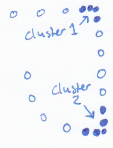
\includegraphics[width=1in]{img/corner-clusters.png}
    \caption{Clusters of high curvature.}
    \label{fig:corner-clusters}
  \end{subfigure}
  \hspace{1cm} % spacing, do what you need
  \begin{subfigure}[t]{0.4\textwidth}
    \centering
    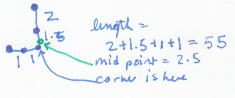
\includegraphics[width=2in]{img/corner-isolation.png}
    \caption{Corner point is closest to middle of cluster.}
    \label{fig:corner-isolation}
  \end{subfigure}
  \caption[Corner finding]{Corner finding involves clustering nearby
    points with high curvature, and choosing the point closest to the
    curvilinear middle of each cluster.}
  \label{fig:corner-finding}
\end{figure}
